\documentclass{article}
\usepackage{amsmath}
\usepackage{listings}
\usepackage{xcolor}
\usepackage{graphicx}
\usepackage{geometry}
\usepackage{hyperref}
\usepackage{tikz}
\usetikzlibrary{trees, positioning}
\geometry{margin=1in}

\title{Graph Algorithms}
\author{}
\date{}

\definecolor{codegray}{rgb}{0.5,0.5,0.5}
\definecolor{backcolour}{rgb}{0.95,0.95,0.92}

\lstdefinestyle{cppstyle}{
  backgroundcolor=\color{backcolour},
  commentstyle=\color{codegray},
  keywordstyle=\color{blue},
  numberstyle=\tiny\color{codegray},
  stringstyle=\color{red},
  basicstyle=\ttfamily\footnotesize,
  breakatwhitespace=false,
  breaklines=true,
  captionpos=b,
  keepspaces=true,
  numbers=none,
  numbersep=5pt,
  showspaces=false,
  showstringspaces=false,
  showtabs=false,
  tabsize=2,
  language=C++
}

\begin{document}

\maketitle


\section{What is a Graph?}

A \textbf{graph} is a mathematical structure used to model pairwise relations between objects. A graph $G$ consists of:
\begin{itemize}
    \item A set of \textbf{vertices} (or nodes), $V$.
    \item A set of \textbf{edges}, $E$, representing connections between pairs of vertices.
\end{itemize}

Graphs may be:
\begin{itemize}
    \item \textbf{Undirected} or \textbf{Directed}
    \item \textbf{Weighted} or \textbf{Unweighted}
    \item \textbf{Cyclic} or \textbf{Acyclic}
    \item \textbf{Connected} or \textbf{Disconnected}
\end{itemize}

\section{Why Graphs?}

Graphs are widely used in:
\begin{itemize}
    \item Computer networks (routers as vertices, links as edges)
    \item Social networks (people as vertices, relationships as edges)
    \item Maps and GPS routing (cities and roads)
    \item Scheduling and dependency analysis
\end{itemize}

\section{Example Graph}

\begin{center}
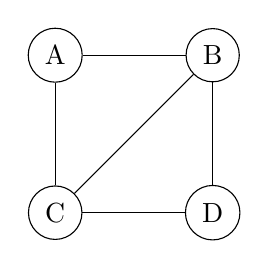
\begin{tikzpicture}[node distance=2cm, every node/.style={circle, draw}]
    \node (A) {A};
    \node (B) [right of=A] {B};
    \node (C) [below of=A] {C};
    \node (D) [right of=C] {D};
    \draw (A) -- (B);
    \draw (A) -- (C);
    \draw (B) -- (D);
    \draw (C) -- (D);
    \draw (B) -- (C);
\end{tikzpicture}
\end{center}

\section{Common Terminology}

\begin{itemize}
    \item \textbf{Vertex (Node):} A point in the graph.
    \item \textbf{Edge:} A connection between two vertices.
    \item \textbf{Degree:} Number of edges incident to a vertex.
    \item \textbf{Path:} A sequence of edges connecting a sequence of vertices.
    \item \textbf{Cycle:} A path that begins and ends at the same vertex.
    \item \textbf{Connected Graph:} A graph where there's a path between any two vertices.
\end{itemize}

\section{Directed vs. Undirected Graphs}

\begin{itemize}
    \item In an \textbf{undirected graph}, edges have no direction. An edge $(u, v)$ implies that $u$ is connected to $v$ and vice versa.
    \item In a \textbf{directed graph (digraph)}, each edge has a direction. An edge $(u, v)$ goes from $u$ to $v$ only.
\end{itemize}

\subsection*{Edge Weights}

Some graphs associate a numerical value (called a \textbf{weight}) with each edge. These are known as \textbf{weighted graphs}. Weights might represent distances, costs, capacities, etc.

\subsection*{Illustration}

\begin{center}
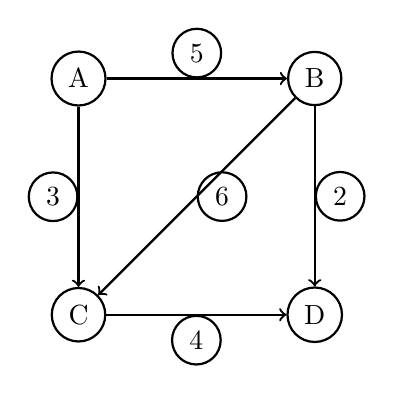
\begin{tikzpicture}[->, thick, node distance=3cm, every node/.style={circle, draw}]
    % Nodes
    \node (A) {A};
    \node (B) [right of=A] {B};
    \node (C) [below of=A] {C};
    \node (D) [right of=C] {D};

    % Directed edges with weights
    \draw[->] (A) -- (B) node[midway, above] {5};
    \draw[->] (A) -- (C) node[midway, left] {3};
    \draw[->] (C) -- (D) node[midway, below] {4};
    \draw[->] (B) -- (D) node[midway, right] {2};
    \draw[->] (B) -- (C) node[midway, right] {6};
\end{tikzpicture}
\end{center}

\textbf{Notes:}
\begin{itemize}
    \item The arrows indicate that the graph is directed.
    \item Numbers on the edges represent weights.
    \item If the same edges had no arrows and were bidirectional, it would represent an undirected weighted graph.
\end{itemize}

\section{Graph Representation}

\textbf{1. Adjacency Matrix}

\begin{itemize}
    \item A 2D matrix of size $n \times n$, where $n$ is the number of vertices.
    \item Entry $(i, j)$ is 1 (or weight $w$) if there is an edge from $i$ to $j$.
\end{itemize}

\begin{lstlisting}[style=cppstyle]
// Adjacency Matrix Representation
int n = 4; // number of vertices
vector<vector<int>> adjMatrix(n, vector<int>(n, 0));

// Add edge between u and v
adjMatrix[u][v] = 1;
adjMatrix[v][u] = 1; // if undirected
\end{lstlisting}

\textbf{2. Adjacency List}

\begin{itemize}
    \item An array of lists, where index $i$ stores the list of adjacent vertices to $i$.
    \item More space-efficient for sparse graphs.
\end{itemize}

\begin{lstlisting}[style=cppstyle]
// Adjacency List Representation
int n = 4; // number of vertices
vector<vector<int>> adjList(n);

// Add edge between u and v
adjList[u].push_back(v);
adjList[v].push_back(u); // if undirected
\end{lstlisting}

\section{Breadth-First Search (BFS)}

\textbf{BFS} explores a graph level by level, using a queue. It is useful for finding the shortest path in unweighted graphs.

\begin{lstlisting}[style=cppstyle]
// BFS from source vertex
void bfs(int src, vector<vector<int>>& adj, int n) {
    vector<bool> visited(n, false);
    queue<int> q;
    
    visited[src] = true;
    q.push(src);

    while (!q.empty()) {
        int node = q.front(); q.pop();
        cout << node << " ";

        for (int neighbor : adj[node]) {
            if (!visited[neighbor]) {
                visited[neighbor] = true;
                q.push(neighbor);
            }
        }
    }
}
\end{lstlisting}

\textbf{Time Complexity:} $O(V + E)$

\section{Depth-First Search (DFS)}

\textbf{DFS} explores as far as possible along a branch before backtracking. It can be implemented recursively or using a stack.

\begin{lstlisting}[style=cppstyle]
// DFS using recursion
void dfs(int node, vector<vector<int>>& adj, vector<bool>& visited) {
    visited[node] = true;
    cout << node << " ";

    for (int neighbor : adj[node]) {
        if (!visited[neighbor]) {
            dfs(neighbor, adj, visited);
        }
    }
}
\end{lstlisting}

\textbf{Time Complexity:} $O(V + E)$

\section{Applications of BFS and DFS}

\subsection{BFS for Unweighted Shortest Path}

Breadth-First Search (BFS) can be used to compute the shortest path from a source vertex to all other vertices in an \textbf{unweighted graph}.

The idea is that BFS explores vertices in layers: it visits all nodes at distance 1 before distance 2, and so on. Thus, the first time we visit a node, we've found the shortest path to it in terms of number of edges.

\begin{lstlisting}[style=cppstyle]
// Compute shortest path from source using BFS
vector<int> bfsShortestPath(int src, const vector<vector<int>>& adj, int n) {
    vector<int> dist(n, -1);  // -1 indicates unreachable
    queue<int> q;

    dist[src] = 0;
    q.push(src);

    while (!q.empty()) {
        int u = q.front(); q.pop();
        for (int v : adj[u]) {
            if (dist[v] == -1) {
                dist[v] = dist[u] + 1;
                q.push(v);
            }
        }
    }
    return dist;
}
\end{lstlisting}

\textbf{Note:} This approach does not handle edge weights. Use Dijkstra’s algorithm if weights are involved.

\subsection{Checking Graph Connectivity}

To determine if a graph is \textbf{connected}, we can use either BFS or DFS:

\begin{itemize}
    \item Start from any node and perform BFS or DFS.
    \item After traversal, check if all nodes were visited.
\end{itemize}

\begin{lstlisting}[style=cppstyle]
// Simple DFS function for connectivity
void dfs(int u, const vector<vector<int>>& adj, vector<bool>& visited, int& count) {
    visited[u] = true;
    count++;
    for (int v : adj[u]) {
        if (!visited[v]) {
            dfs(v, adj, visited, count);
        }
    }
}

// Returns true if the graph is connected
bool isConnected(const vector<vector<int>>& adj, int n) {
    vector<bool> visited(n, false);
    int count = 0;

    dfs(0, adj, visited, count); // Start from node 0

    return count == n;
}
\end{lstlisting}

\textbf{Note on Directed Graphs:}
\begin{itemize}
    \item A directed graph is \textbf{strongly connected} if there is a path from every vertex to every other vertex following the direction of edges.
    \item It is \textbf{weakly connected} if the graph is connected when edge directions are ignored (i.e., treated as undirected).
\end{itemize}

Determining strong connectivity requires more advanced algorithms such as Kosaraju’s or Tarjan’s algorithm.

\subsection{Topological Sorting via DFS}

Topological sorting is applicable to \textbf{Directed Acyclic Graphs (DAGs)}. It produces a linear ordering of vertices such that for every directed edge $(u \rightarrow v)$, vertex $u$ appears before $v$ in the ordering.

DFS-based topological sorting:
\begin{itemize}
    \item Perform DFS on the graph.
    \item On finishing a node, push it to a stack or prepend to a list.
    \item Reverse the result at the end.
\end{itemize}

\begin{lstlisting}[style=cppstyle]
// Topological sort using DFS
void topoDFS(int u, vector<vector<int>>& adj, vector<bool>& visited, vector<int>& result) {
    visited[u] = true;
    for (int v : adj[u]) {
        if (!visited[v])
            topoDFS(v, adj, visited, result);
    }
    result.push_back(u); // Add after visiting children
}

vector<int> topologicalSort(int n, vector<vector<int>>& adj) {
    vector<bool> visited(n, false);
    vector<int> result;

    for (int i = 0; i < n; ++i) {
        if (!visited[i])
            topoDFS(i, adj, visited, result);
    }

    reverse(result.begin(), result.end());
    return result;
}
\end{lstlisting}

\subsection{Spanning Trees and BFS/DFS Construction}

A \textbf{spanning tree} of a connected, undirected graph is a subgraph that:
\begin{itemize}
    \item Includes all the vertices of the original graph,
    \item Is a tree (i.e., contains no cycles),
    \item Has exactly $n - 1$ edges if there are $n$ vertices.
\end{itemize}

Spanning trees are fundamental in graph theory and network design (e.g., building minimum-cost networks without cycles).

\textbf{Key Property:} Every connected undirected graph has at least one spanning tree.

\subsubsection*{Constructing a Spanning Tree Using BFS}

You can build a spanning tree by performing a BFS and recording the edges used to first discover each vertex.

\begin{lstlisting}[style=cppstyle]
// Returns list of edges in the BFS spanning tree
vector<pair<int, int>> bfsSpanningTree(int start, const vector<vector<int>>& adj, int n) {
    vector<bool> visited(n, false);
    vector<pair<int, int>> treeEdges;
    queue<int> q;

    visited[start] = true;
    q.push(start);

    while (!q.empty()) {
        int u = q.front(); q.pop();
        for (int v : adj[u]) {
            if (!visited[v]) {
                visited[v] = true;
                treeEdges.push_back({u, v});
                q.push(v);
            }
        }
    }

    return treeEdges;
}
\end{lstlisting}

\subsubsection*{Constructing a Spanning Tree Using DFS}

Likewise, DFS can be used to form a spanning tree by recording edges used during the traversal.

\begin{lstlisting}[style=cppstyle]
// Returns list of edges in the DFS spanning tree
void dfsSpanningTree(int u, const vector<vector<int>>& adj, vector<bool>& visited,
                     vector<pair<int, int>>& treeEdges) {
    visited[u] = true;
    for (int v : adj[u]) {
        if (!visited[v]) {
            treeEdges.push_back({u, v});
            dfsSpanningTree(v, adj, visited, treeEdges);
        }
    }
}
\end{lstlisting}

To use:
\begin{lstlisting}[style=cppstyle]
vector<bool> visited(n, false);
vector<pair<int, int>> treeEdges;
dfsSpanningTree(0, adj, visited, treeEdges);
\end{lstlisting}

\textbf{Note:} These methods generate \textit{some} spanning tree, not necessarily a minimum spanning tree (MST). For MSTs, use Prim’s or Kruskal’s algorithm.

\section{Advanced Graph Algorithms: Greedy Approach}

Many important graph problems can be solved efficiently using the \textbf{greedy paradigm}, where a local optimal choice is made at each step with the hope that it leads to a global optimum.

Two key graph algorithms based on this idea are:
\begin{itemize}
    \item \textbf{Prim’s Algorithm} for finding a Minimum Spanning Tree (MST),
    \item \textbf{Dijkstra’s Algorithm} for finding the shortest path from a source node.
\end{itemize}

\subsection{Prim’s Algorithm: Minimum Spanning Tree}

Prim’s algorithm constructs a \textbf{minimum spanning tree} by growing the tree one edge at a time. At each step, it adds the minimum weight edge that connects a vertex in the tree to a vertex outside the tree.

\textbf{Greedy Principle:} At each step, choose the lightest edge that expands the tree without forming a cycle.

\begin{lstlisting}[style=cppstyle]
// Prim's algorithm without priority queue
vector<int> primMST(const vector<vector<pair<int, int>>>& adj, int n) {
    vector<bool> inMST(n, false);
    vector<int> key(n, INT_MAX);  // Minimum weight to include node
    vector<int> parent(n, -1);    // Store MST edges
    key[0] = 0;

    for (int count = 0; count < n; ++count) {
        // Find the vertex u not in MST with minimum key[u]
        int u = -1;
        for (int i = 0; i < n; ++i) {
            if (!inMST[i] && (u == -1 || key[i] < key[u]))
                u = i;
        }

        inMST[u] = true;

        for (auto [v, weight] : adj[u]) {
            if (!inMST[v] && weight < key[v]) {
                key[v] = weight;
                parent[v] = u;
            }
        }
    }

    return parent; // parent[i] gives the MST edge to i
}
\end{lstlisting}

\textbf{Time Complexity:} $O(V^2)$ due to the repeated minimum selection via linear scan.


\textbf{Time Complexity:} $O((V + E) \log V)$ with a priority queue.  
\textbf{Input:} Undirected, connected, weighted graph.

\subsection{Dijkstra’s Algorithm: Single-Source Shortest Path}

Dijkstra’s algorithm finds the shortest path from a source vertex to all other vertices in a graph with non-negative edge weights.

\textbf{Greedy Principle:} At each step, pick the closest unvisited vertex and update distances to its neighbors.

\begin{lstlisting}[style=cppstyle]
// Dijkstra's algorithm without priority queue
vector<int> dijkstra(int src, const vector<vector<pair<int, int>>>& adj, int n) {
    vector<int> dist(n, INT_MAX);
    vector<bool> visited(n, false);
    dist[src] = 0;

    for (int count = 0; count < n; ++count) {
        // Find unvisited vertex u with smallest dist[u]
        int u = -1;
        for (int i = 0; i < n; ++i) {
            if (!visited[i] && (u == -1 || dist[i] < dist[u]))
                u = i;
        }

        visited[u] = true;

        for (auto [v, weight] : adj[u]) {
            if (dist[u] + weight < dist[v]) {
                dist[v] = dist[u] + weight;
            }
        }
    }

    return dist;
}
\end{lstlisting}

\textbf{Time Complexity:} $O(V^2)$ — acceptable for dense graphs or small inputs.


\subsection{Why Greedy Works}

Both Prim's and Dijkstra's algorithms build solutions incrementally:
\begin{itemize}
    \item They always pick the next node or edge that seems best \textit{at the moment}.
    \item They avoid revisiting or backtracking once a decision is made.
    \item Correctness is guaranteed due to the properties of MSTs (Prim) and non-negative weights (Dijkstra).
\end{itemize}

\subsection{How Heaps Improve Efficiency}

Both Prim’s and Dijkstra’s algorithms involve repeatedly selecting the vertex with the smallest key/distance. This operation is costly with a linear scan ($O(V)$ per iteration).

By using a \textbf{min-heap (priority queue)}, we reduce this selection time to $O(\log V)$:
\begin{itemize}
    \item \textbf{Prim's with heap:} $O((V + E) \log V)$
    \item \textbf{Dijkstra with heap:} $O((V + E) \log V)$
\end{itemize}

\section{Other Graph Algorithms (Brief Overview)}

\begin{itemize}
    \item \textbf{Kruskal’s Algorithm:} Greedy algorithm for finding a minimum spanning tree using edge sorting and union-find.
    \item \textbf{Bellman-Ford Algorithm:} Computes shortest paths from a source, allowing negative edge weights.
    \item \textbf{Floyd-Warshall Algorithm:} Computes all-pairs shortest paths using dynamic programming.
    \item \textbf{Topological Sort (Kahn’s Algorithm):} Iterative method to produce a topological ordering of a DAG.
    \item \textbf{Kosaraju’s Algorithm:} Detects strongly connected components in a directed graph.
    \item \textbf{Tarjan’s Algorithm:} Finds strongly connected components in a single DFS traversal.
    \item \textbf{Union-Find (Disjoint Set Union):} Efficient structure for handling connectivity queries and cycle detection.
    \item \textbf{Hamiltonian Cycle:} A cycle that visits each vertex exactly once and returns to the starting vertex.
    \item \textbf{Eulerian Cycle:} A cycle that visits every edge exactly once and returns to the start (exists if all degrees are even in an undirected graph).
\end{itemize}

\end{document}